\documentclass[11pt]{report}
\clubpenalty=10000
\widowpenalty=10000

% It is handy to define new commands for text that occurs frequently (see Discussion)
\newcommand{\MT}{^{\mathrm{MT}}}
\newcommand{\ga}{\gtrsim}
\newcommand{\Lpot}{(L+1)^2}
\newcommand{\WS}{^{\mathrm{WS}}}


%--Format the section headers

\input{packages}
% FJS Changed this... I didn't like the numbering or the
% indentation... so I introduced a fake chapter Main Text. 
\setcounter{secnumdepth}{0}
\setcounter{tocdepth}{5}

% Add pandoc command wrapper macro thing (?)
\makeatletter
\newsavebox\pandoc@box
\newcommand*\pandocbounded[1]{%
  \sbox\pandoc@box{#1}%
  % scaling factors for width and height
  \Gscale@div\@tempa\textheight{\dimexpr\ht\pandoc@box+\dp\pandoc@box\relax}%
  \Gscale@div\@tempb\linewidth{\wd\pandoc@box}%
  % select the smaller of both
  \ifdim\@tempb\p@<\@tempa\p@
    \let\@tempa\@tempb
  \fi
  % scaling accordingly (\@tempa < 1)
  \ifdim\@tempa\p@<\p@
    \scalebox{\@tempa}{\usebox\pandoc@box}%
  % scaling not needed, use as it is
  \else
    \usebox{\pandoc@box}%
  \fi
}
\makeatother

%--set the page formatting--
\geometry{hmargin={1.6in,1.1in},vmargin={1.5in,1.2in}}
\doublespacing

% allow code to be shwon in shaded r markdown environment

% add csl referencing capacity and styling

\begin{document}
%--front matter needs roman pagination--
\pagenumbering{roman}

%--Title Page--
\thispagestyle{empty}
  \begin{center}
    \textsc{\LARGE Senior Thesis} %Fill in your information
  \end{center}
  \vspace{.6in}
  \begin{center}
    Collin R. Guedel
  \end{center}
  \vspace{.6in}
  \begin{center}
    \textsc{A Senior Thesis \\ %Fill in your information
    Presented to the Faculty \\
    of Princeton University \\
    in Candidacy for the Degree \\
    of Bachelor of Arts}
  \end{center}
  \vspace{.3in}
  \begin{center}
    \textsc{Recommended for Acceptance \\
    by the Department of \\
    Geosciences \\}
    Advisor: Professor Xinning Zhang %Fill in your information
  \end{center}
  \vspace{.3in}
  \begin{center}
    02 April, 2026 %Fill in your information
  \end{center}
  
  \clearpage

%--Copyright Page--
\thispagestyle{empty}
\vspace*{3in}
\begin{center}
\emph{This paper represents my own work in accordance with University regulations,} \\
Collin R. Guedel
\end{center}
\clearpage

%--Abstract-- 
%\phantomsection
\addcontentsline{toc}{chapter}{Abstract}
\begin{center}
\Large \textbf{Abstract}
\end{center}
 Human land use, primarily through farming and its resulting land disturbances impacts the soil sink of atmospheric hydrogen maintained by soil microbial communities; this thesis' aim is to assess, both through measurements of soil H2 uptake rate and bacterial genomics, what governs this rate. Based upon preliminary agricultural data that I assess this summer, it appears that tilling has a significant impact on agricultural soils' uptake ; I would like to study this further by comparing farming practices and the resultant microbial behaviors in comparison to undisturbed, non-agriculture soils.
 \clearpage

%--Acknowledgements--
%\phantomsection
\addcontentsline{toc}{chapter}{Acknowledgements}
\begin{center}
\Large \textbf{Acknowledgements}
\end{center}
Thanks Mom and Dad!
\clearpage

%--Table of Contents--  
\thispagestyle{empty}
\tableofcontents
\clearpage

\listoffigures
\listoftables
%\clearpage

%--Set up fancy header-- 
\fancyhead{}
\fancyfoot{}
\pagestyle{fancyplain}
\rhead{\fancyplain{\thepage}{\noindent \textsc{\rightmark} \hfill \thepage~of~\pageref{LastPage}}}
\rfoot{\hrule \today \hfill Collin R. Guedel}
\pagenumbering{arabic}
\setlength{\headheight}{13.59999pt}.

%--Reset the page numbers and set them to arabic-- 
{\newpage\renewcommand{\thepage}{\arabic{page}}\setcounter{page}{1}}

%--Have sections but use chapter counters
%\phantomsection
\addcontentsline{toc}{chapter}{Main Text}

\newpage

\section{Introduction}\label{introduction}

TBD
\citet{sandMultimodelAssessmentGlobal2023} says

\section{Methods}\label{methods}

\([H_2] = [H_2]_{eq} + ([H_2]_0-[H_2]_{eq})e^{-kt}\)

\begin{verbatim}
## Warning: Removed 6 rows containing missing values or values outside the scale range
## (`geom_point()`).
\end{verbatim}

\begin{center}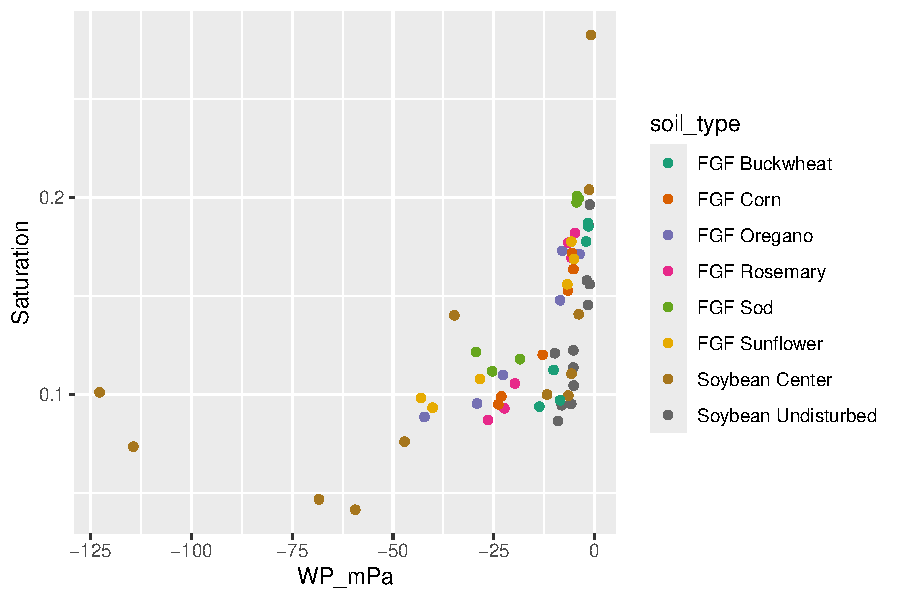
\includegraphics{The-Thesis_files/figure-latex/soil_metadata-1} \end{center}

\section{Results}\label{results}

\subsection{Summer Data}\label{summer-data}

\begin{verbatim}
## New names:
## * `` -> `...16`
## * `` -> `...18`
## * `` -> `...21`
\end{verbatim}

\begin{center}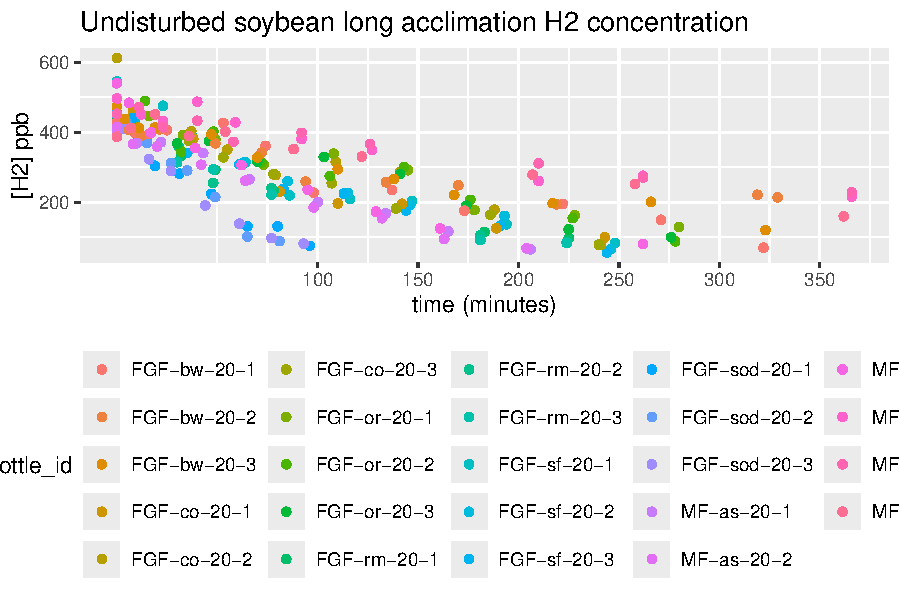
\includegraphics{The-Thesis_files/figure-latex/summer_plots-1} \end{center}

\begin{center}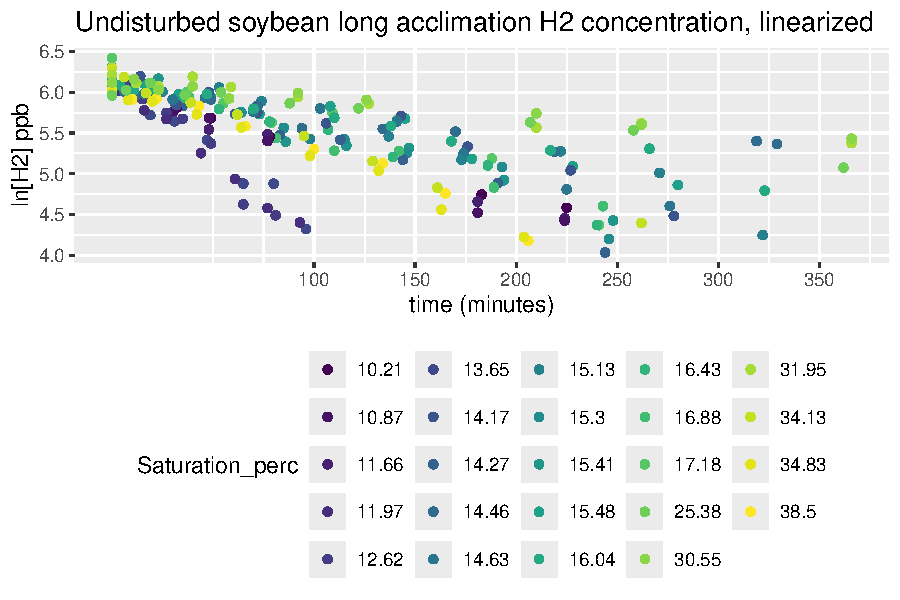
\includegraphics{The-Thesis_files/figure-latex/summer_plots-2} \end{center}

\begin{verbatim}
## `geom_smooth()` using formula = 'y ~ x'
\end{verbatim}

\begin{center}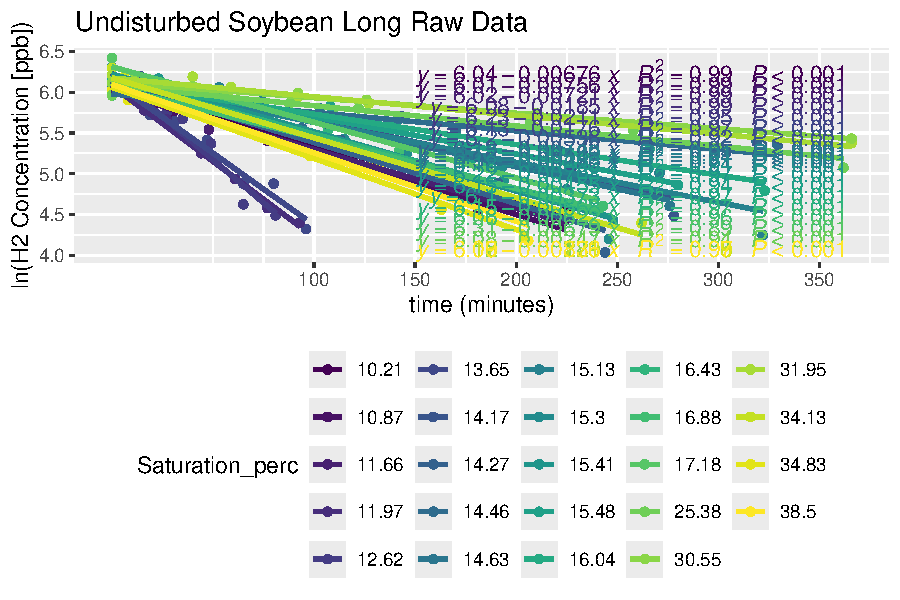
\includegraphics{The-Thesis_files/figure-latex/summer_plots-3} \end{center}

\begin{verbatim}
## Warning: `fortify(<lm>)` was deprecated in ggplot2 4.0.0.
## i Please use `broom::augment(<lm>)` instead.
## i The deprecated feature was likely used in the ggplot2 package.
##   Please report the issue at <https://github.com/tidyverse/ggplot2/issues>.
## This warning is displayed once every 8 hours.
## Call `lifecycle::last_lifecycle_warnings()` to see where this warning was
## generated.
\end{verbatim}

\begin{center}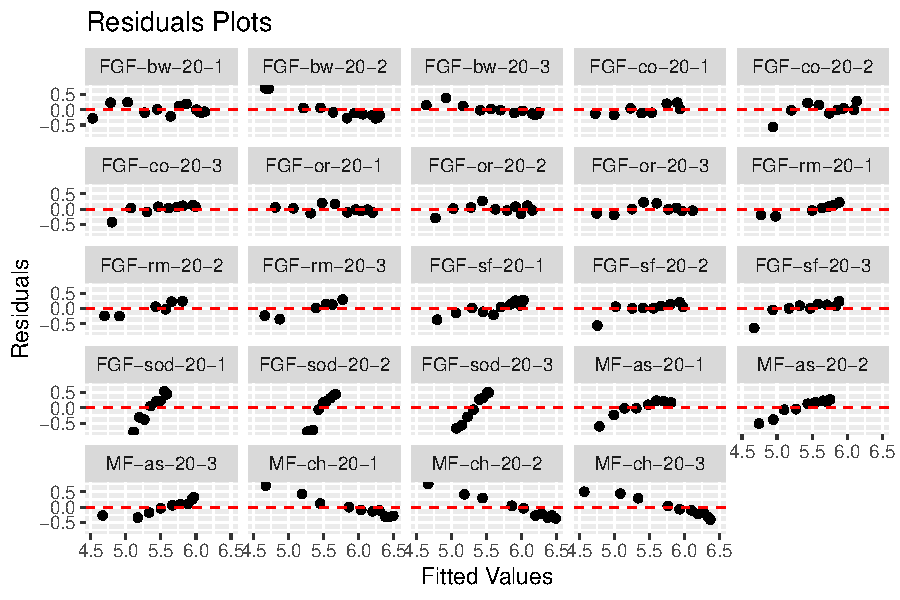
\includegraphics{The-Thesis_files/figure-latex/summer_plots-4} \end{center}

\subsection{Soy - Undisturbed - Long}\label{soy---undisturbed---long}

\begin{center}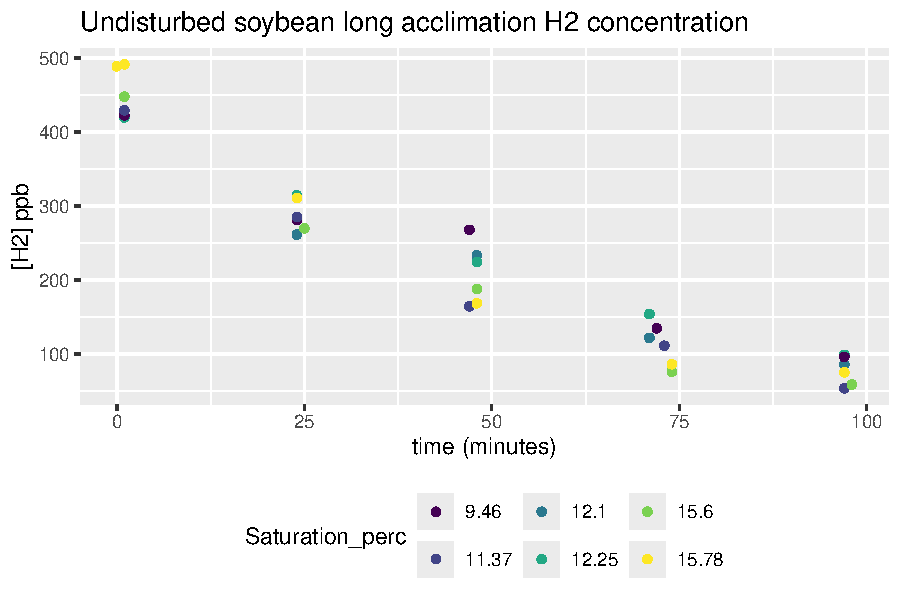
\includegraphics{The-Thesis_files/figure-latex/Long-Soy-UD Plots-1} \end{center}

\begin{center}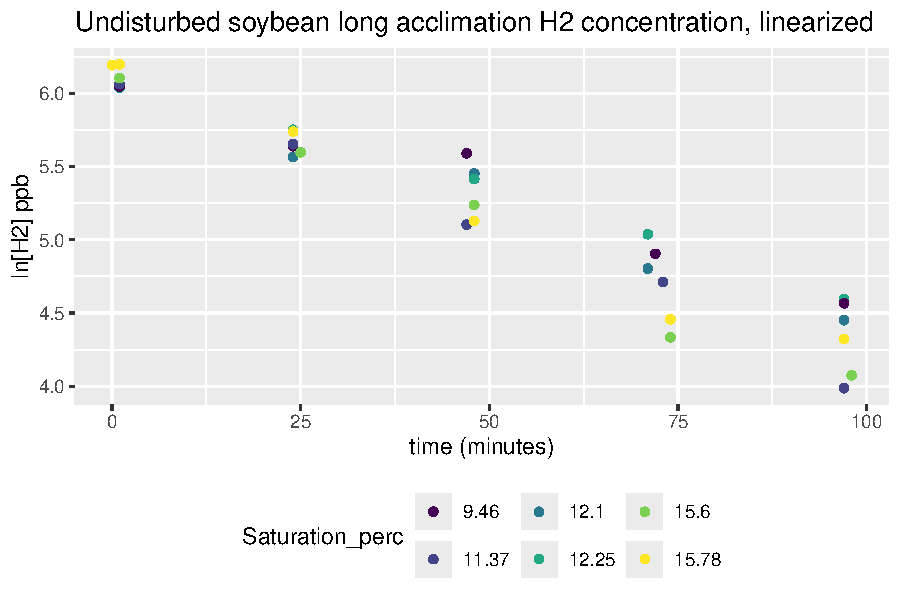
\includegraphics{The-Thesis_files/figure-latex/Long-Soy-UD Plots-2} \end{center}

\begin{verbatim}
## `geom_smooth()` using formula = 'y ~ x'
\end{verbatim}

\begin{center}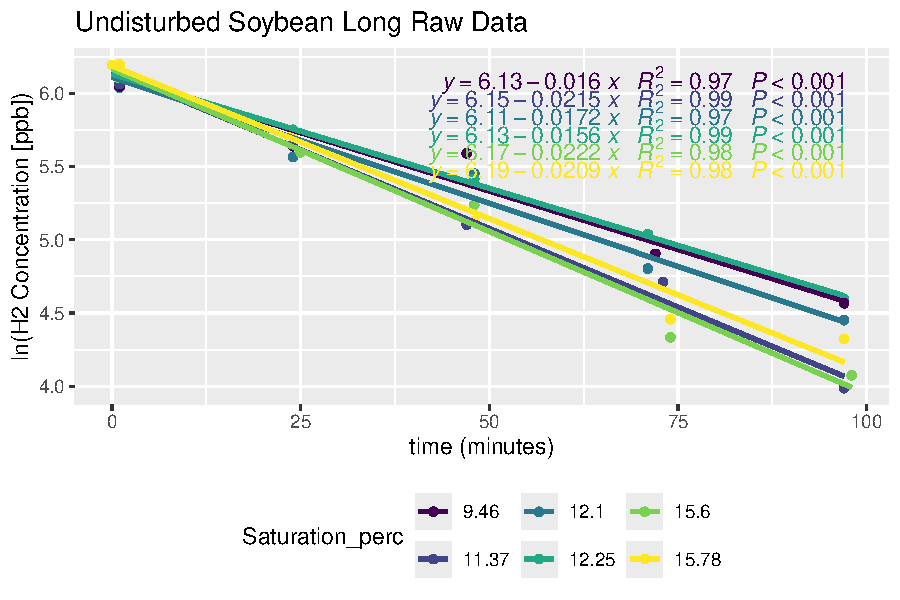
\includegraphics{The-Thesis_files/figure-latex/Long-Soy-UD Plots-3} \end{center}

\begin{center}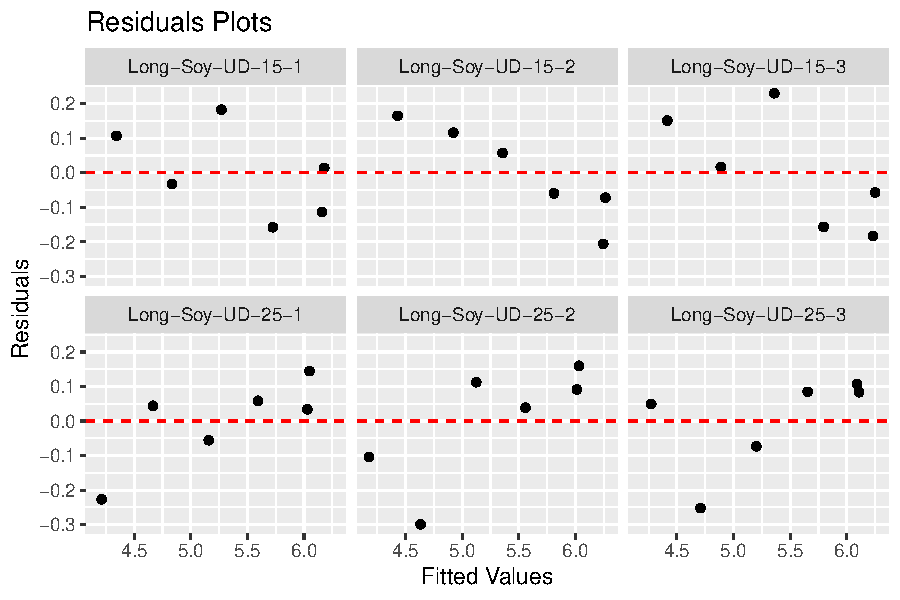
\includegraphics{The-Thesis_files/figure-latex/Long-Soy-UD Plots-4} \end{center}

Of note: The fits are really good here, with very small residuals and R\^{}2 values. The linearization seems to be effective without accounting for the asymptotic behavior near the tails, meaning that equilibrium is not sufficiently reached by the end of these incubation experiments within the time frame. I have included the fitting equations in the graph along with the R\^{}2 values - the p values don't mean much because they only compare these lines to a slope of 0, which is obviously out of the question.

\begin{verbatim}
## Adding missing grouping variables: `bottle_id`
\end{verbatim}

\begin{verbatim}
## Warning: `qplot()` was deprecated in ggplot2 3.4.0.
## This warning is displayed once every 8 hours.
## Call `lifecycle::last_lifecycle_warnings()` to see where this warning was
## generated.
\end{verbatim}

\begin{center}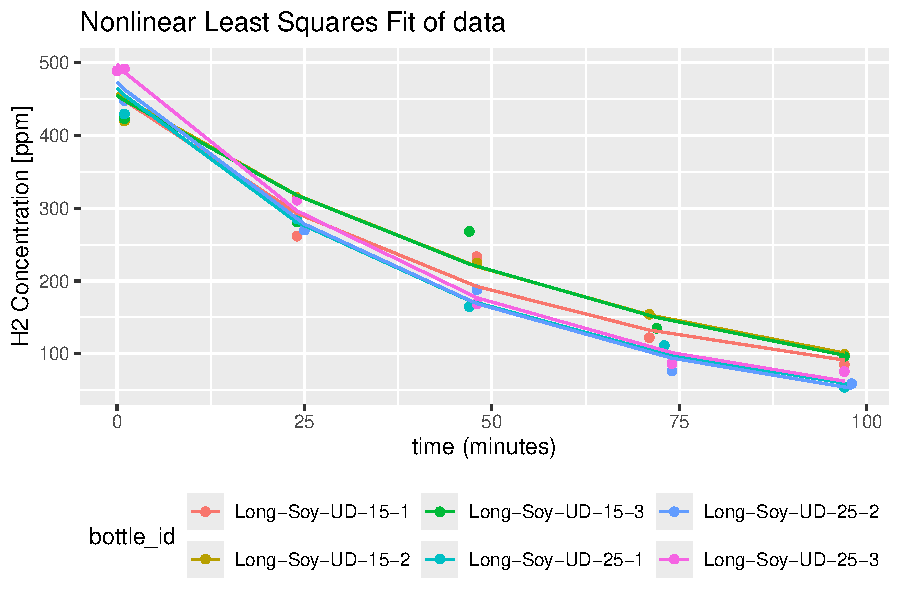
\includegraphics{The-Thesis_files/figure-latex/Long-Soy-UD Fits-1} \end{center}

\begin{verbatim}
## Adding missing grouping variables: `bottle_id`
\end{verbatim}

\begin{center}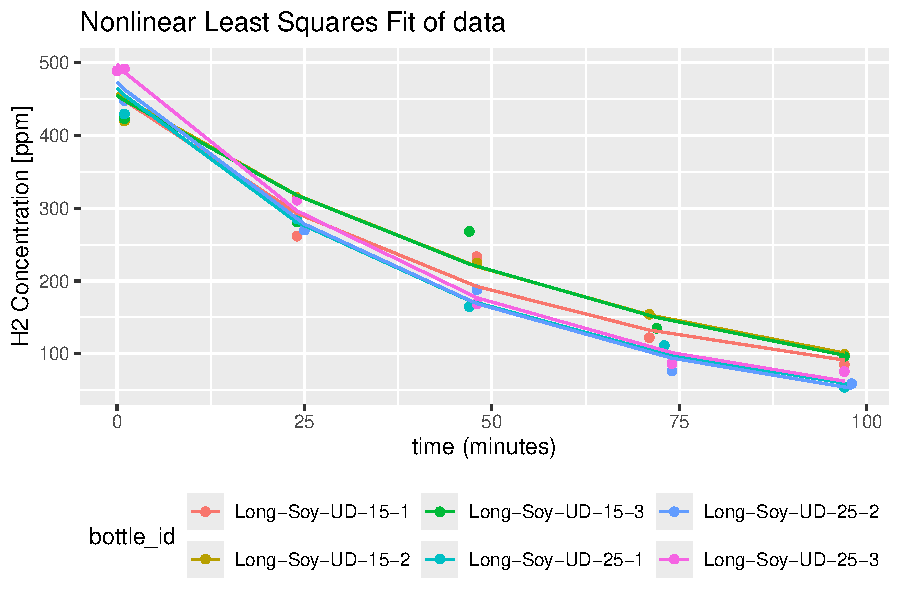
\includegraphics{The-Thesis_files/figure-latex/Long-Soy-UD Fabian Fits-1} \end{center}

This nonlinear fit is less interpretable than the linearized fits seen above, because, as the data tables show, it is often guessing that the asymptote line is below 0 ppb of H2, which is impossible. The earlier linearized fitting methods make more physical sense and don't seem to diverge from linearity based upon the residuals plot, but they \emph{may} seem to diverge from homoscedasticity - the residuals plots for each don't seem totally amorphous, but they may be a result of the very small sample sizes per bottle. Regardless, heteroscedasticity does not introduce bias into the model (it doesn't sway the regression coefficient one way or another), but it does mean our models are less precise than the high R\^{}2 values would make them appear to be.

There are methods that I want to use to seek to address this - the first being a new-to-me method of regression called a robust regression, another being perhaps a background subtraction of the hydrogen background in the nitrogen carrier gas. Most importantly, I think more trial runs will show us how they are behaving at a grander scale and if there are systemic deviations from the assumed linearity of our natural log linearization.

\subsection{Soy - Disturbed Center - Long}\label{soy---disturbed-center---long}

\begin{center}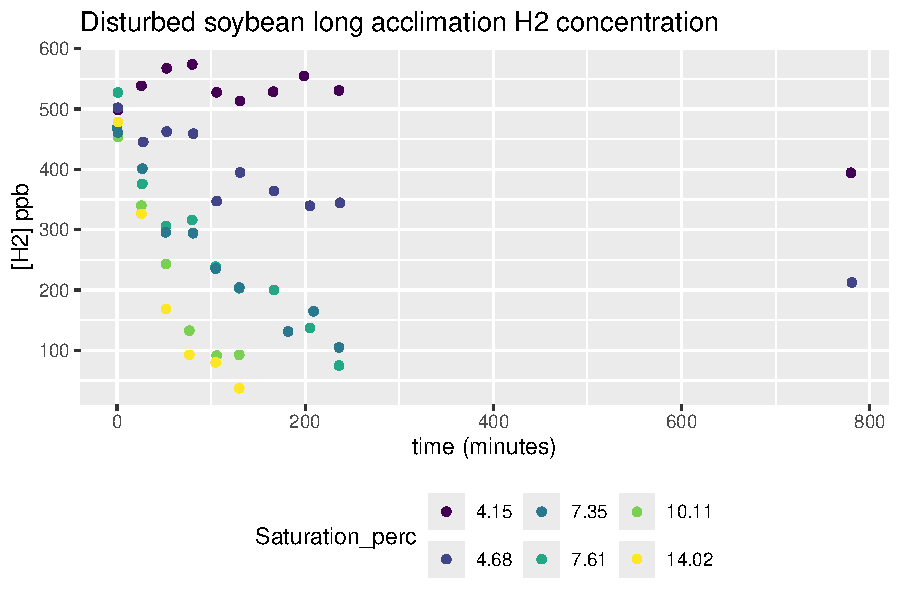
\includegraphics{The-Thesis_files/figure-latex/Long-Soy-C Plots-1} \end{center}

\begin{center}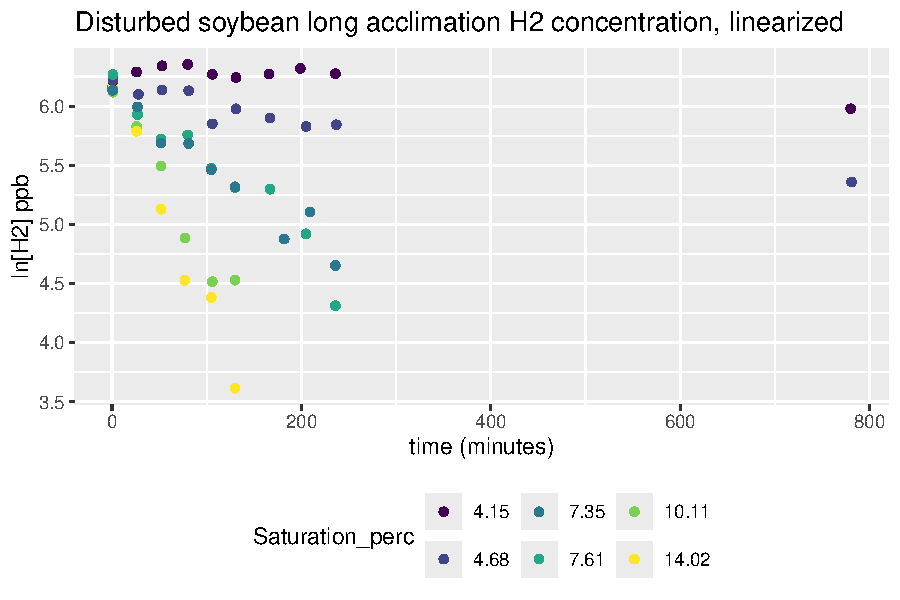
\includegraphics{The-Thesis_files/figure-latex/Long-Soy-C Plots-2} \end{center}

\begin{verbatim}
## `geom_smooth()` using formula = 'y ~ x'
\end{verbatim}

\begin{center}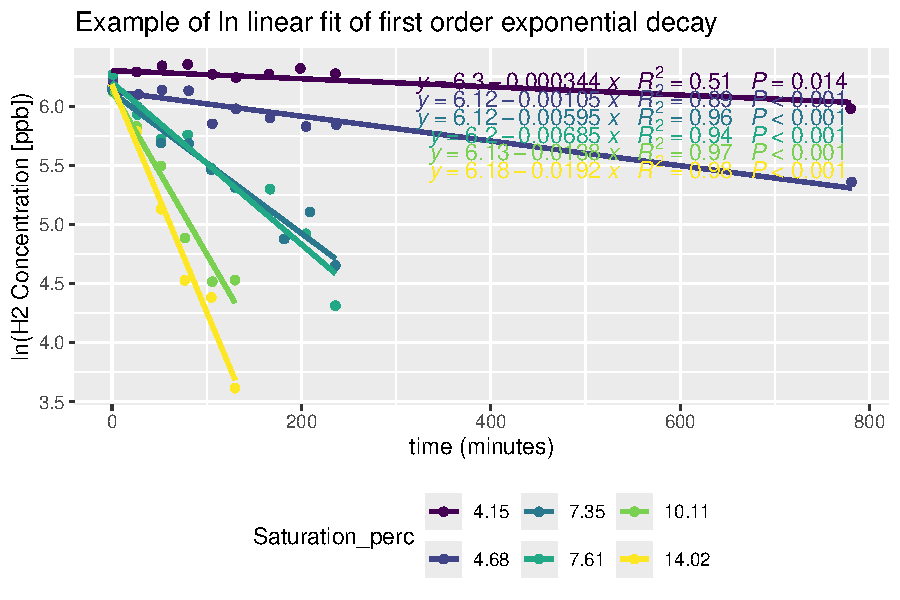
\includegraphics{The-Thesis_files/figure-latex/Long-Soy-C Plots-3} \end{center}

\begin{center}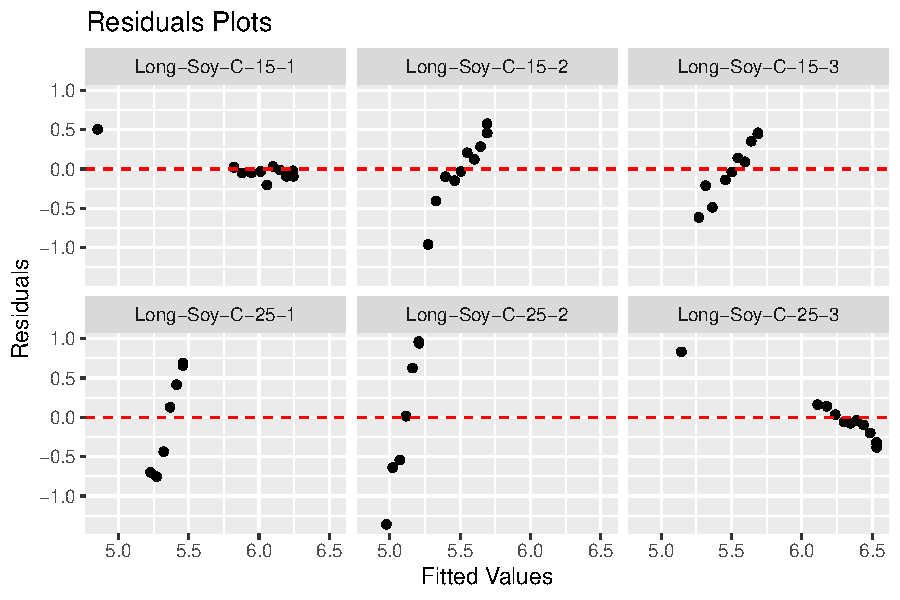
\includegraphics{The-Thesis_files/figure-latex/Long-Soy-C Plots-4} \end{center}

\begin{verbatim}
## Adding missing grouping variables: `bottle_id`
\end{verbatim}

\begin{center}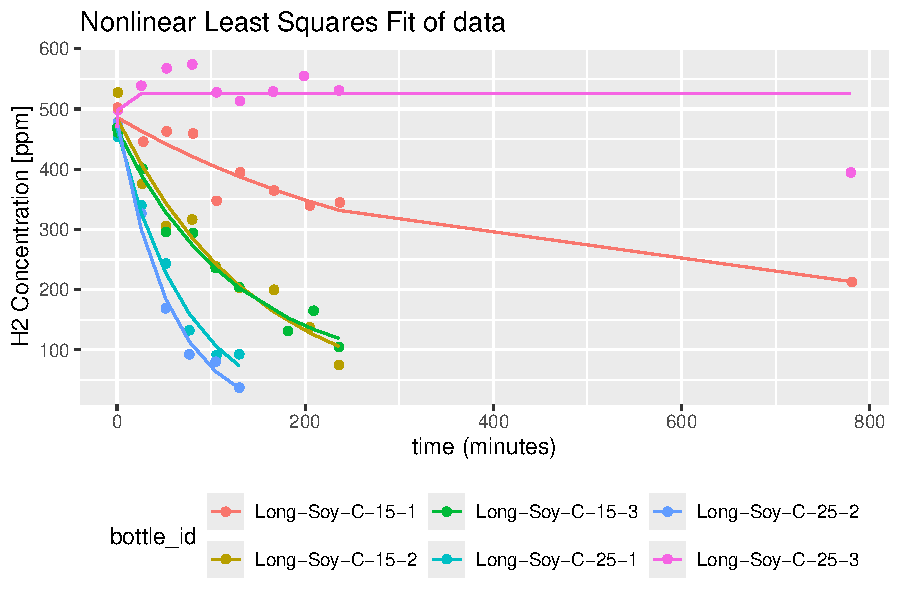
\includegraphics{The-Thesis_files/figure-latex/Long-Soy-C Fits-1} \end{center}

\subsection{Good Soy Runs}\label{good-soy-runs}

\begin{verbatim}
## Adding missing grouping variables: `bottle_id`
\end{verbatim}

\begin{center}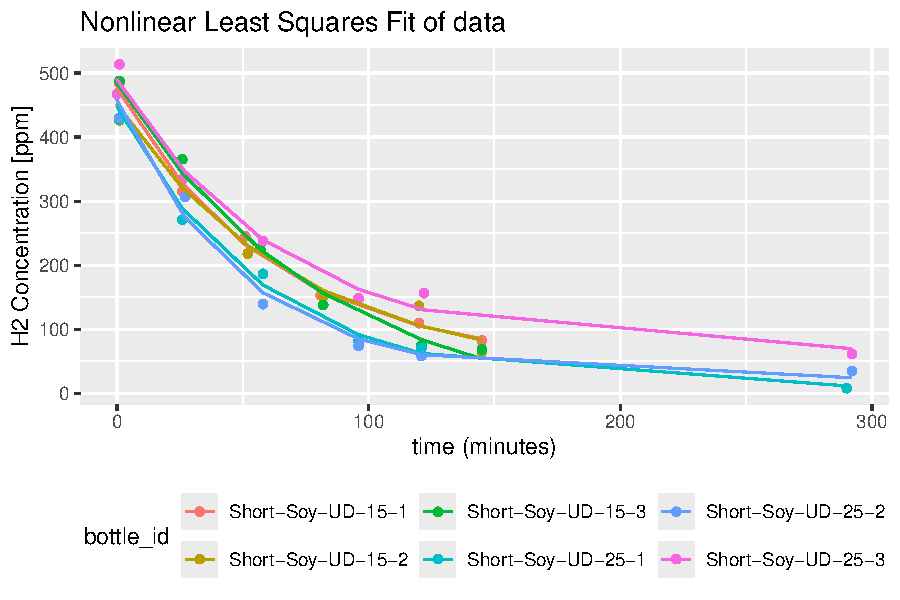
\includegraphics{The-Thesis_files/figure-latex/Short-Soy-UD Fits-1} \end{center}

\begin{verbatim}
## Adding missing grouping variables: `bottle_id`
\end{verbatim}

\begin{center}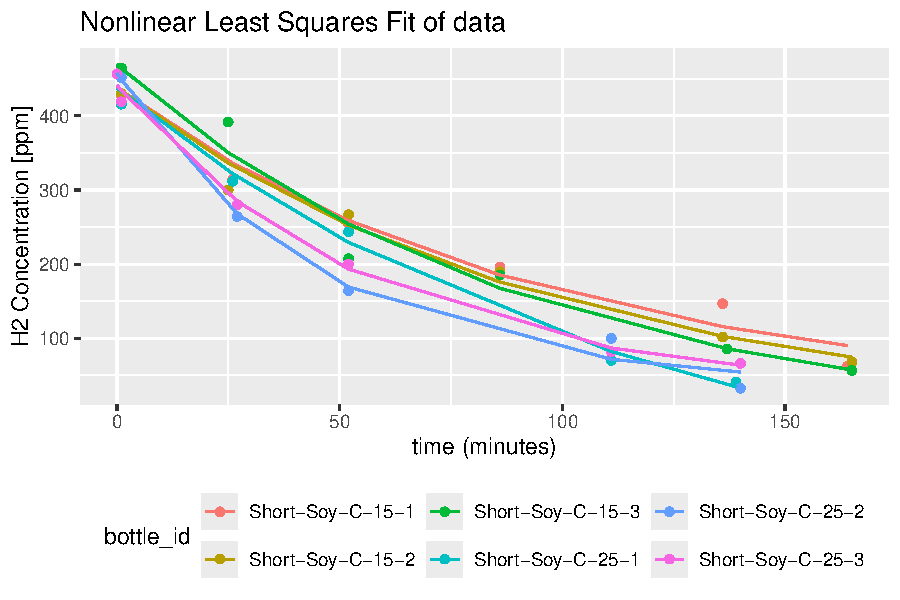
\includegraphics{The-Thesis_files/figure-latex/Short-Soy-C Fits-1} \end{center}

\subsection{Fairgrown Farms}\label{fairgrown-farms}

\begin{verbatim}
## [1] 77
\end{verbatim}

\begin{verbatim}
## Adding missing grouping variables: `bottle_id`
\end{verbatim}

\begin{center}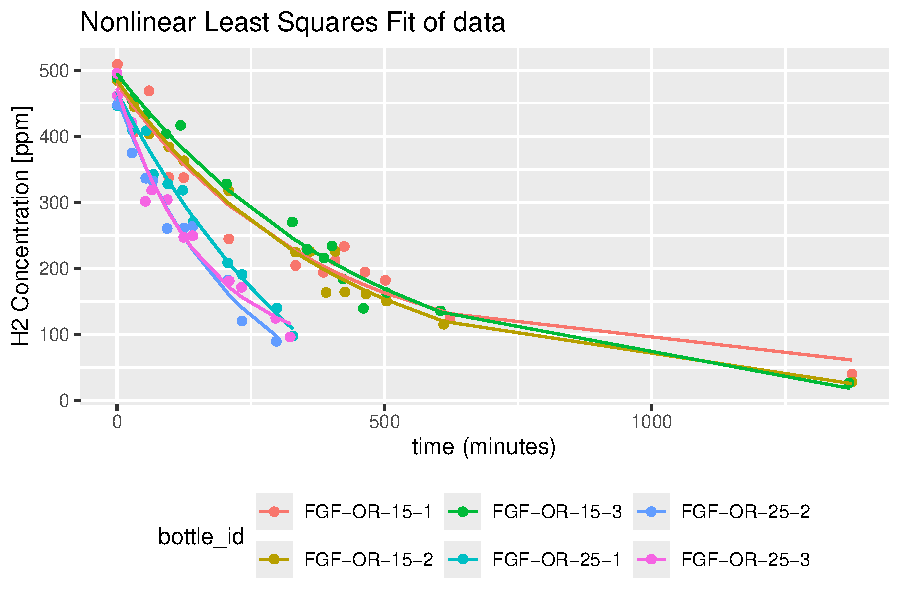
\includegraphics{The-Thesis_files/figure-latex/FGF-OR Fits-1} \end{center}

\begin{verbatim}
## Adding missing grouping variables: `bottle_id`
\end{verbatim}

\begin{center}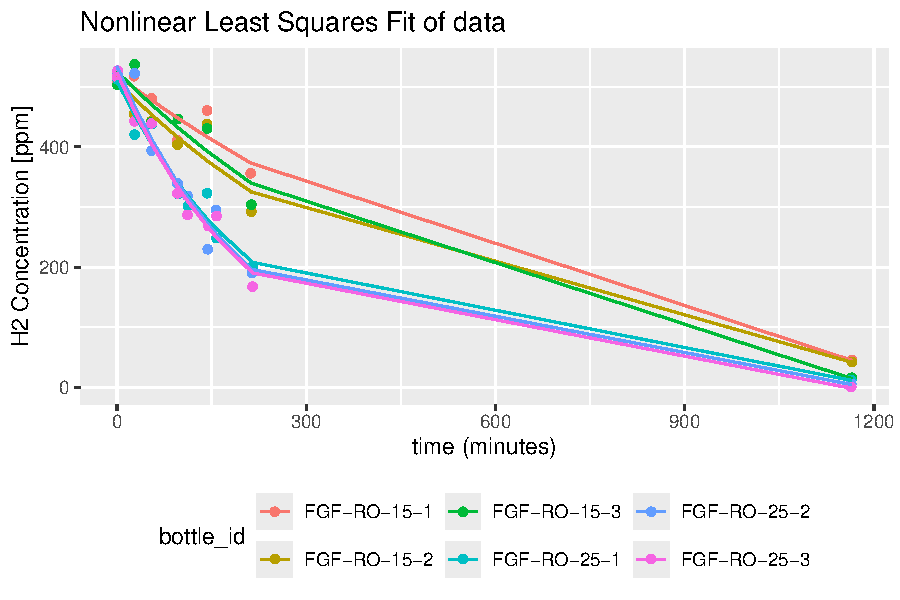
\includegraphics{The-Thesis_files/figure-latex/FGF-RO Fits-1} \end{center}

\begin{verbatim}
## Adding missing grouping variables: `bottle_id`
\end{verbatim}

\begin{center}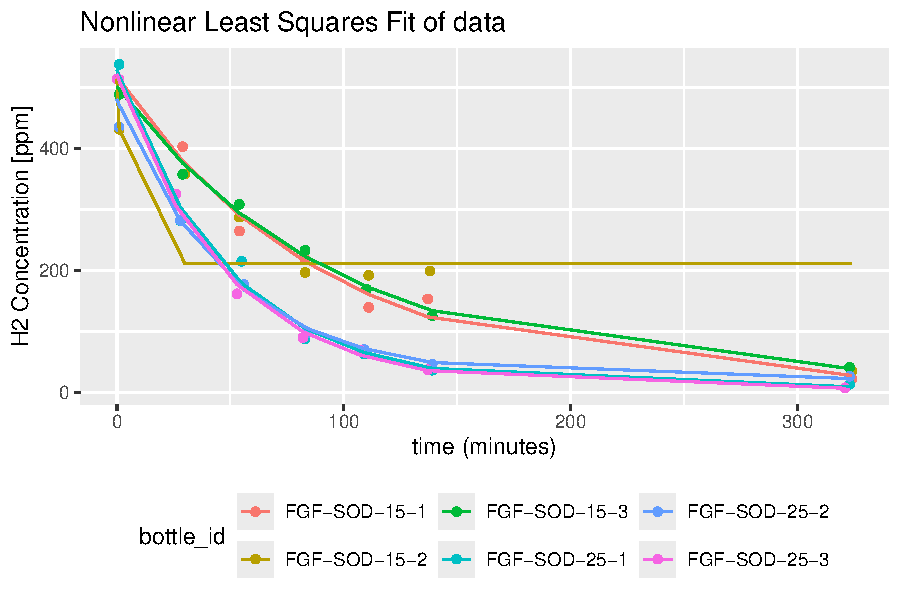
\includegraphics{The-Thesis_files/figure-latex/FGF-SOD Fits-1} \end{center}

\begin{verbatim}
## Adding missing grouping variables: `bottle_id`
\end{verbatim}

\begin{center}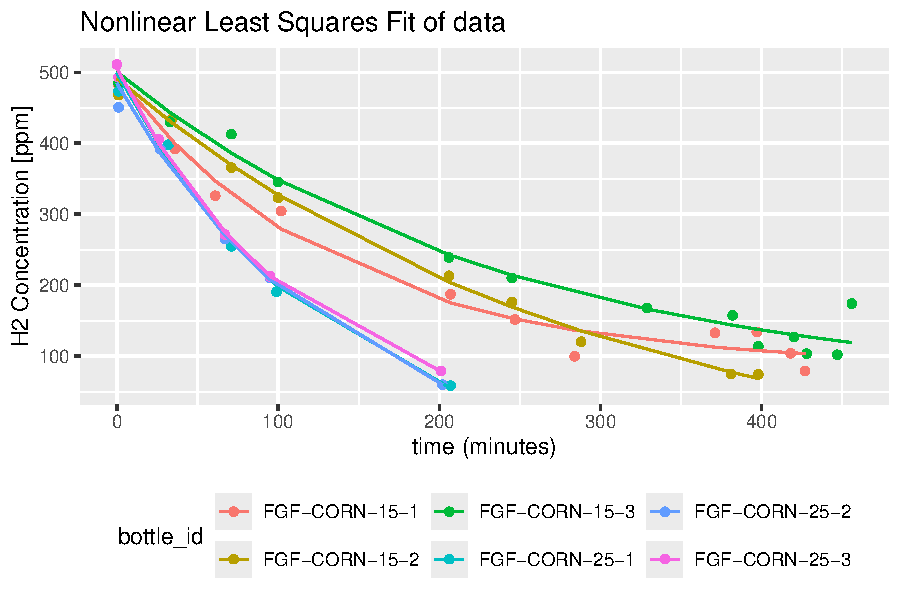
\includegraphics{The-Thesis_files/figure-latex/FGF-CO-N Fits-1} \end{center}

\begin{verbatim}
## Adding missing grouping variables: `bottle_id`
\end{verbatim}

\begin{center}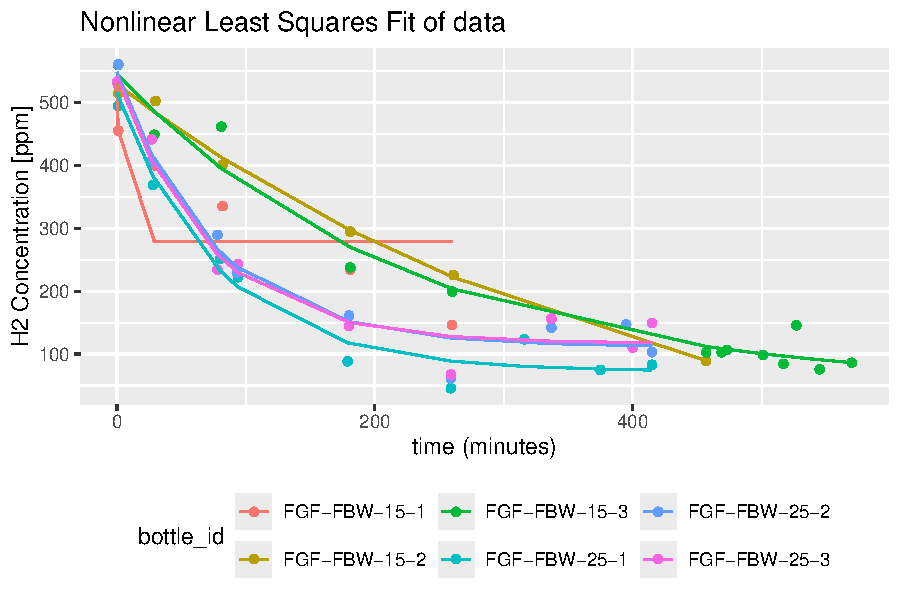
\includegraphics{The-Thesis_files/figure-latex/FGF-FBW-N Fits-1} \end{center}

\begin{verbatim}
## Adding missing grouping variables: `bottle_id`
\end{verbatim}

\begin{center}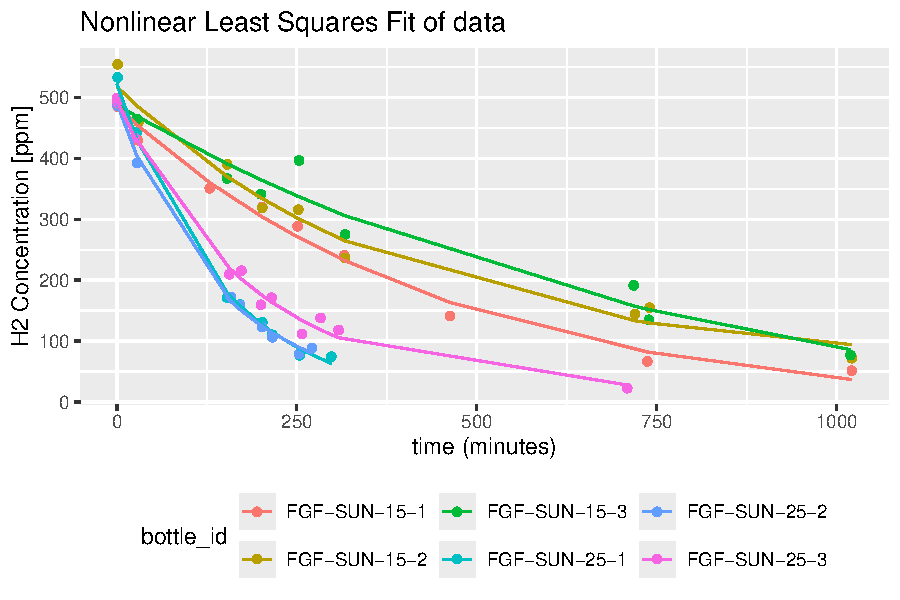
\includegraphics{The-Thesis_files/figure-latex/FGF-SUN-N Fits-1} \end{center}

\subsection{Kinetic Rate Data Summary}\label{kinetic-rate-data-summary}

\begin{verbatim}
## Warning: Removed 6 rows containing missing values or values outside the scale range
## (`geom_point()`).
\end{verbatim}

\begin{center}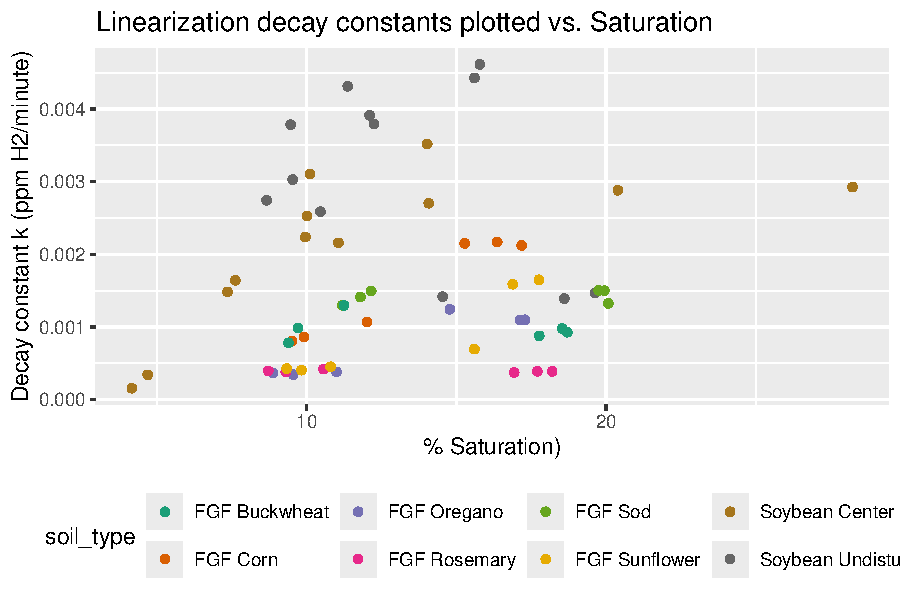
\includegraphics{The-Thesis_files/figure-latex/trial-summaries-1} \end{center}

\begin{verbatim}
## Warning: Removed 6 rows containing missing values or values outside the scale range
## (`geom_point()`).
\end{verbatim}

\begin{center}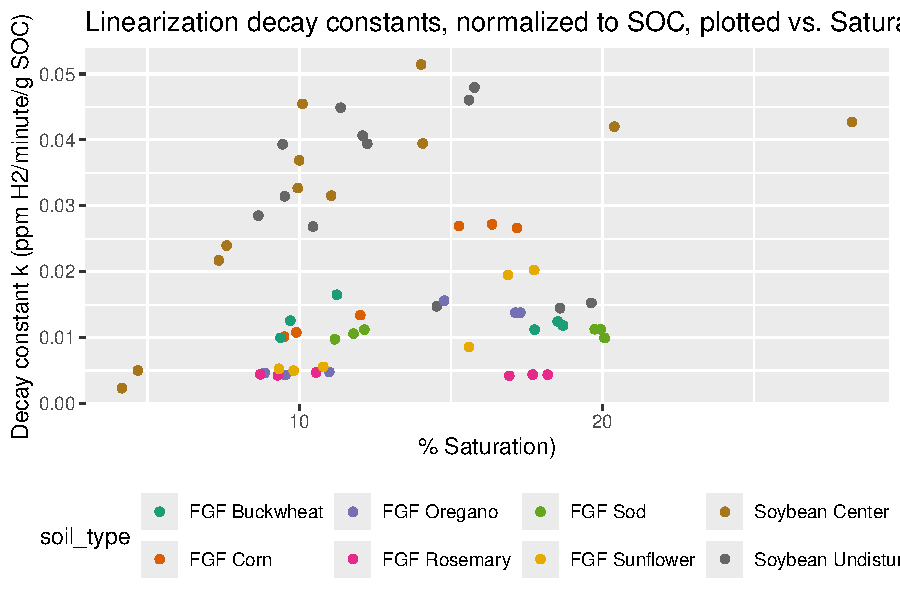
\includegraphics{The-Thesis_files/figure-latex/trial-summaries-2} \end{center}

\begin{verbatim}
## Warning: Removed 6 rows containing missing values or values outside the scale range
## (`geom_point()`).
\end{verbatim}

\begin{center}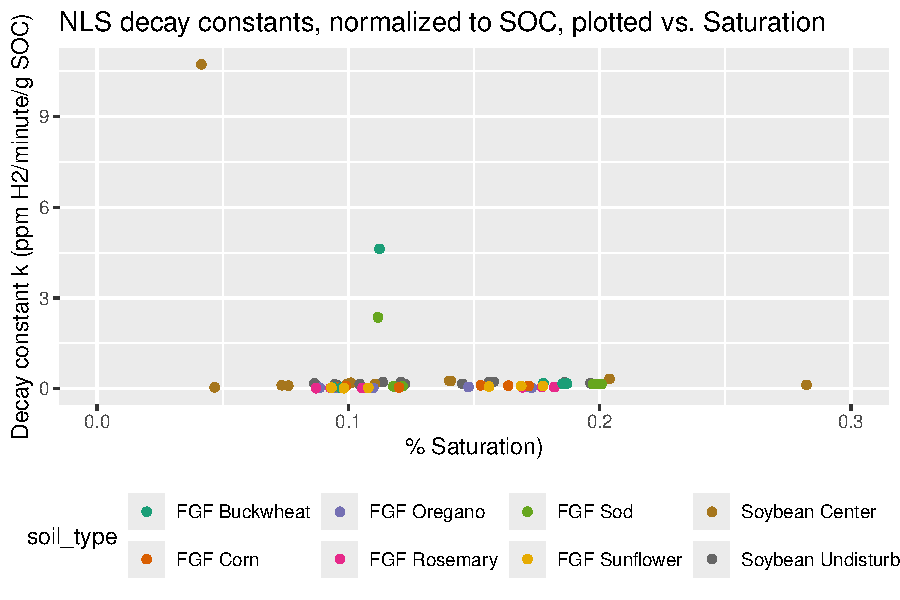
\includegraphics{The-Thesis_files/figure-latex/trial-summaries-3} \end{center}

Include draft work from CEE523 on equation writing.

\section{Discussion}\label{discussion}

\section{Conclusion}\label{conclusion}

\clearpage

\appendix
\appendixpage
\addappheadtotoc

\section{Supplementary Information}\label{supplementary-information}

\section{Code Appendix}\label{code-appendix}

code will go here eventually

%--References--
\small
\renewcommand{\bibsep}{0em}

\renewcommand{\bibname}{References}
\bibliographystyle{gji}
\bibliography{Senior-Thesis-Zhang}
%\printbibliography[heading=none] %Used in biblatex, not natbib


\newpage

%--appendices--

%\appendix
%\appendixpage
%\addappheadtotoc

\end{document}
